\subsection{Comparative analyses of simulation results}

At the start of our different comparative analyses, we will first make a general rough analysis, creating a more simplified and easy-to-understand version of our results. As an example, in figure \ref{Fig:covidInfGraphs}, two histograms are visible, showcasing the only difference in the  simulation, namely the switching of contact tracing (CT). 

In the first histogram(a), the columns clearly show the effect of contact tracing. The maximum number of total infected within thousand drops of our simulation shows no higher than 210 infected of a total 12,500 population size, which equals to 1.68\% being infected of a total population. In other words, contact tracing seems to prove effective, since this is a very low total infection for the population. 

In the second histogram(b), the columns here shows a different reality. If COVID-19 were to run "invisibly", i.e. without society's knowledge and without the preventive measure of contact tracing, the simulation of a thousand drops estimates a maximum of 3857 infected. In comparison to histogram(a), in this simulation of thousand drops without contact tracing, the total infected population can reach as high as 30.8\% of the total population. 

\begin{figure}[H]
 \centering
  \begin{subfigure}{.45\textwidth}
    \centering
    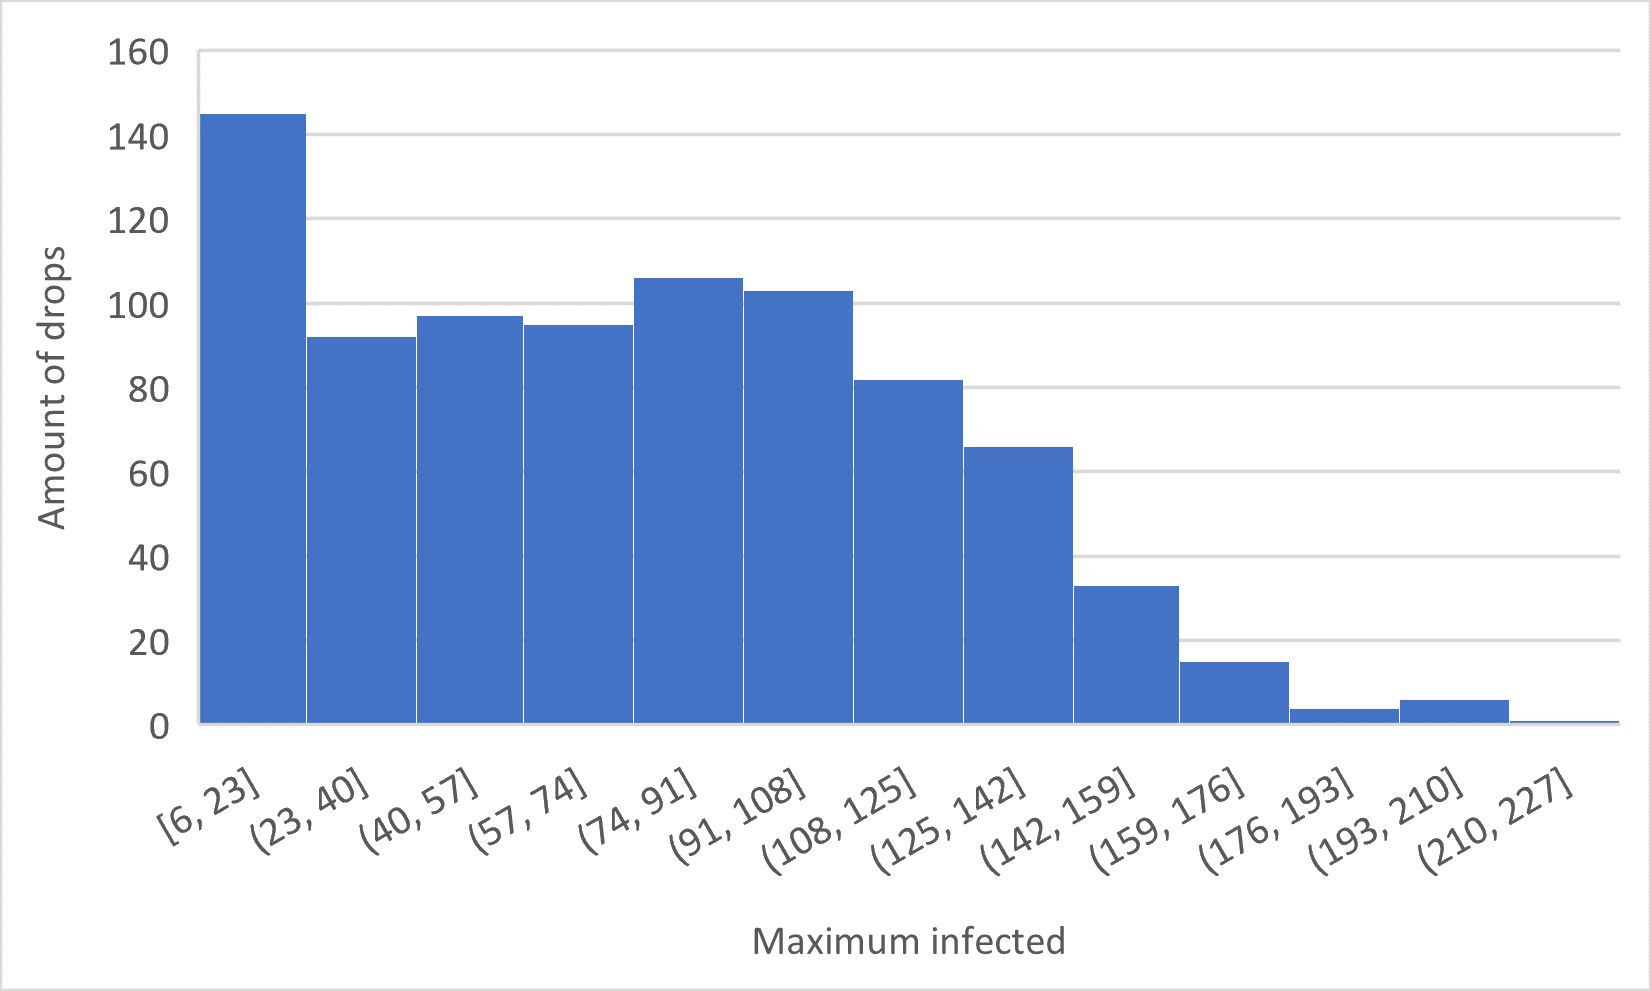
\includegraphics[width=.95\linewidth]{0_billeder/1k_ct_on_graph.png}
    \caption{With contact tracing}
    \label{Subfig:covidInfGraphA}
  \end{subfigure}
  \begin{subfigure}{.45\textwidth}
    \centering
    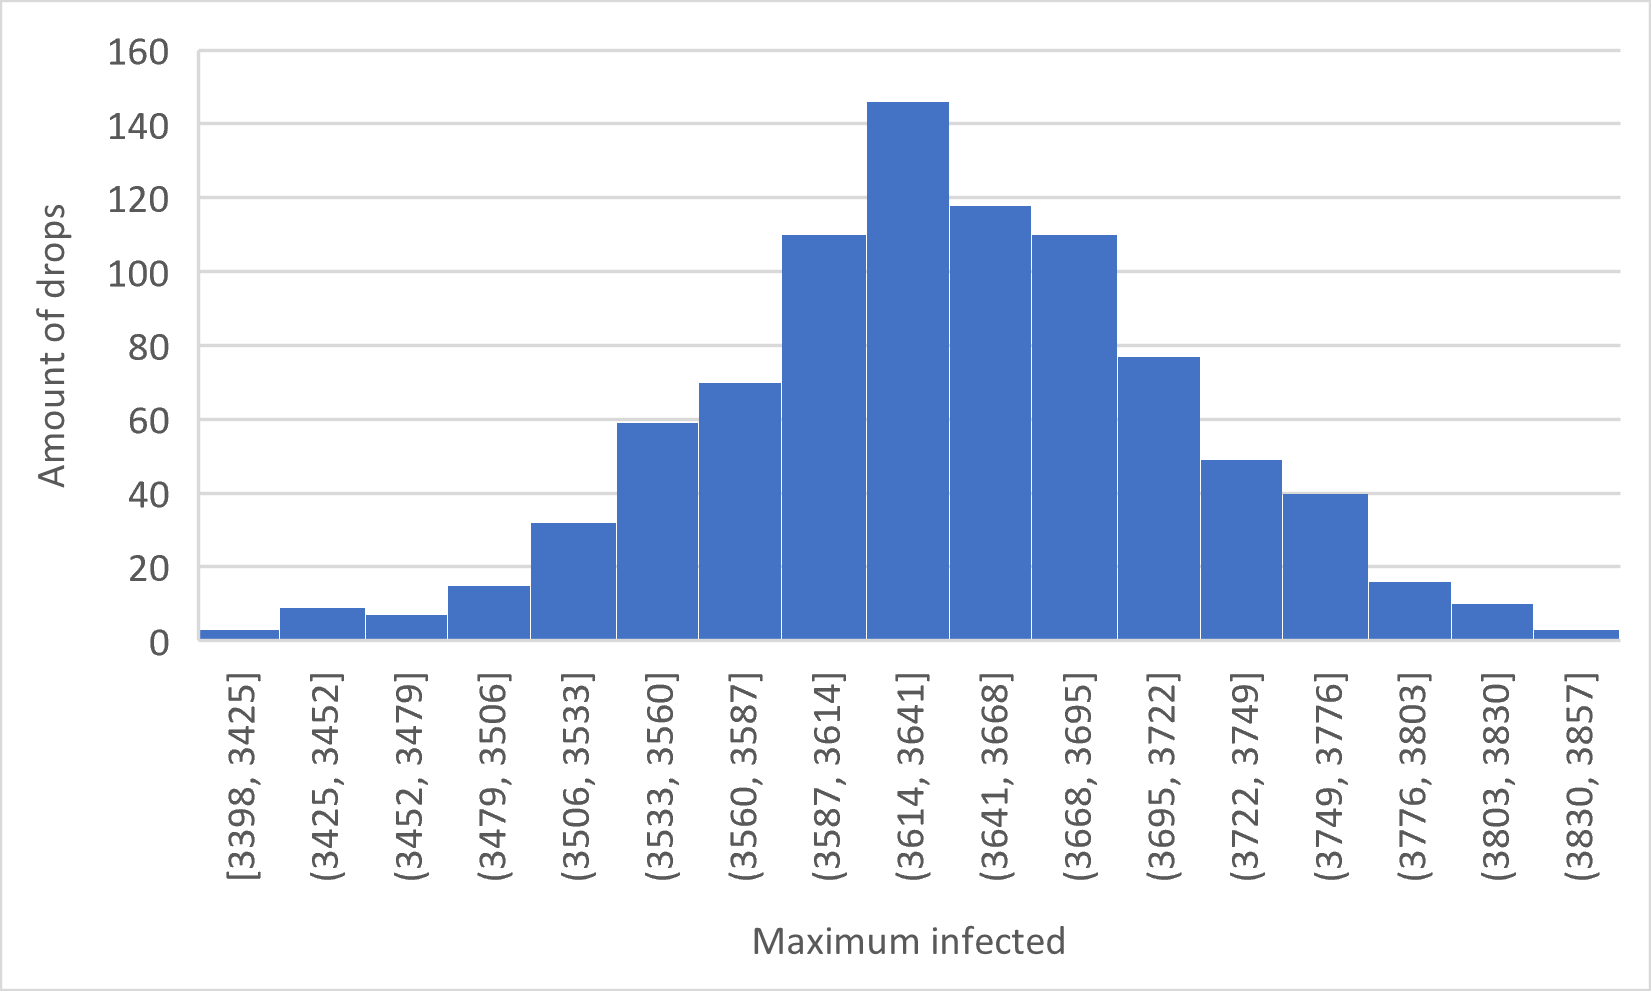
\includegraphics[width=.95\linewidth]{0_billeder/1k_ct_off_graph.png}
    \caption{Without contact tracing}
    \label{Subfig:covidInfGraphB}
  \end{subfigure}
 \caption{Infection histograms with/without contact tracing.}
 \label{Fig:covidInfGraphs}
\end{figure}

Figure \ref{Fig:covidInfGraphs} is a graph of infection, as a function of days, both with- and without contact tracing enabled. Before going into explaining the graphs, it is important to note, that the data used is an average of a thousand drops.

In the first graph with contact tracing disabled, we see that the number of infected people is raising rapidly to its peak which is around 2750 people infected - at day 112. Then the number of infected people quickly drops to 0 again around day 190 and do not change further.

In the second graph, which is with contact tracing enabled, the number of infected also raises rapidly, but it does not reach the same levels as in the first graph. The maximum number of infected in the second graph is around 33 at day 140. After it has peaked, it slowly decrease towards 0, which is reached around day 720.

Comparing the two, it is clear that contact tracing and quarantine is a very effective tool in fighting COVID-19. With contact tracing disabled, the number of infections peak at 2750 people, whereas with contact tracing enabled, it peaks at only 33 people. That corresponds to only 1.2\% of the first graph's peak.

\begin{figure}[H]
 \centering
  \begin{subfigure}{.45\textwidth}
    \centering
    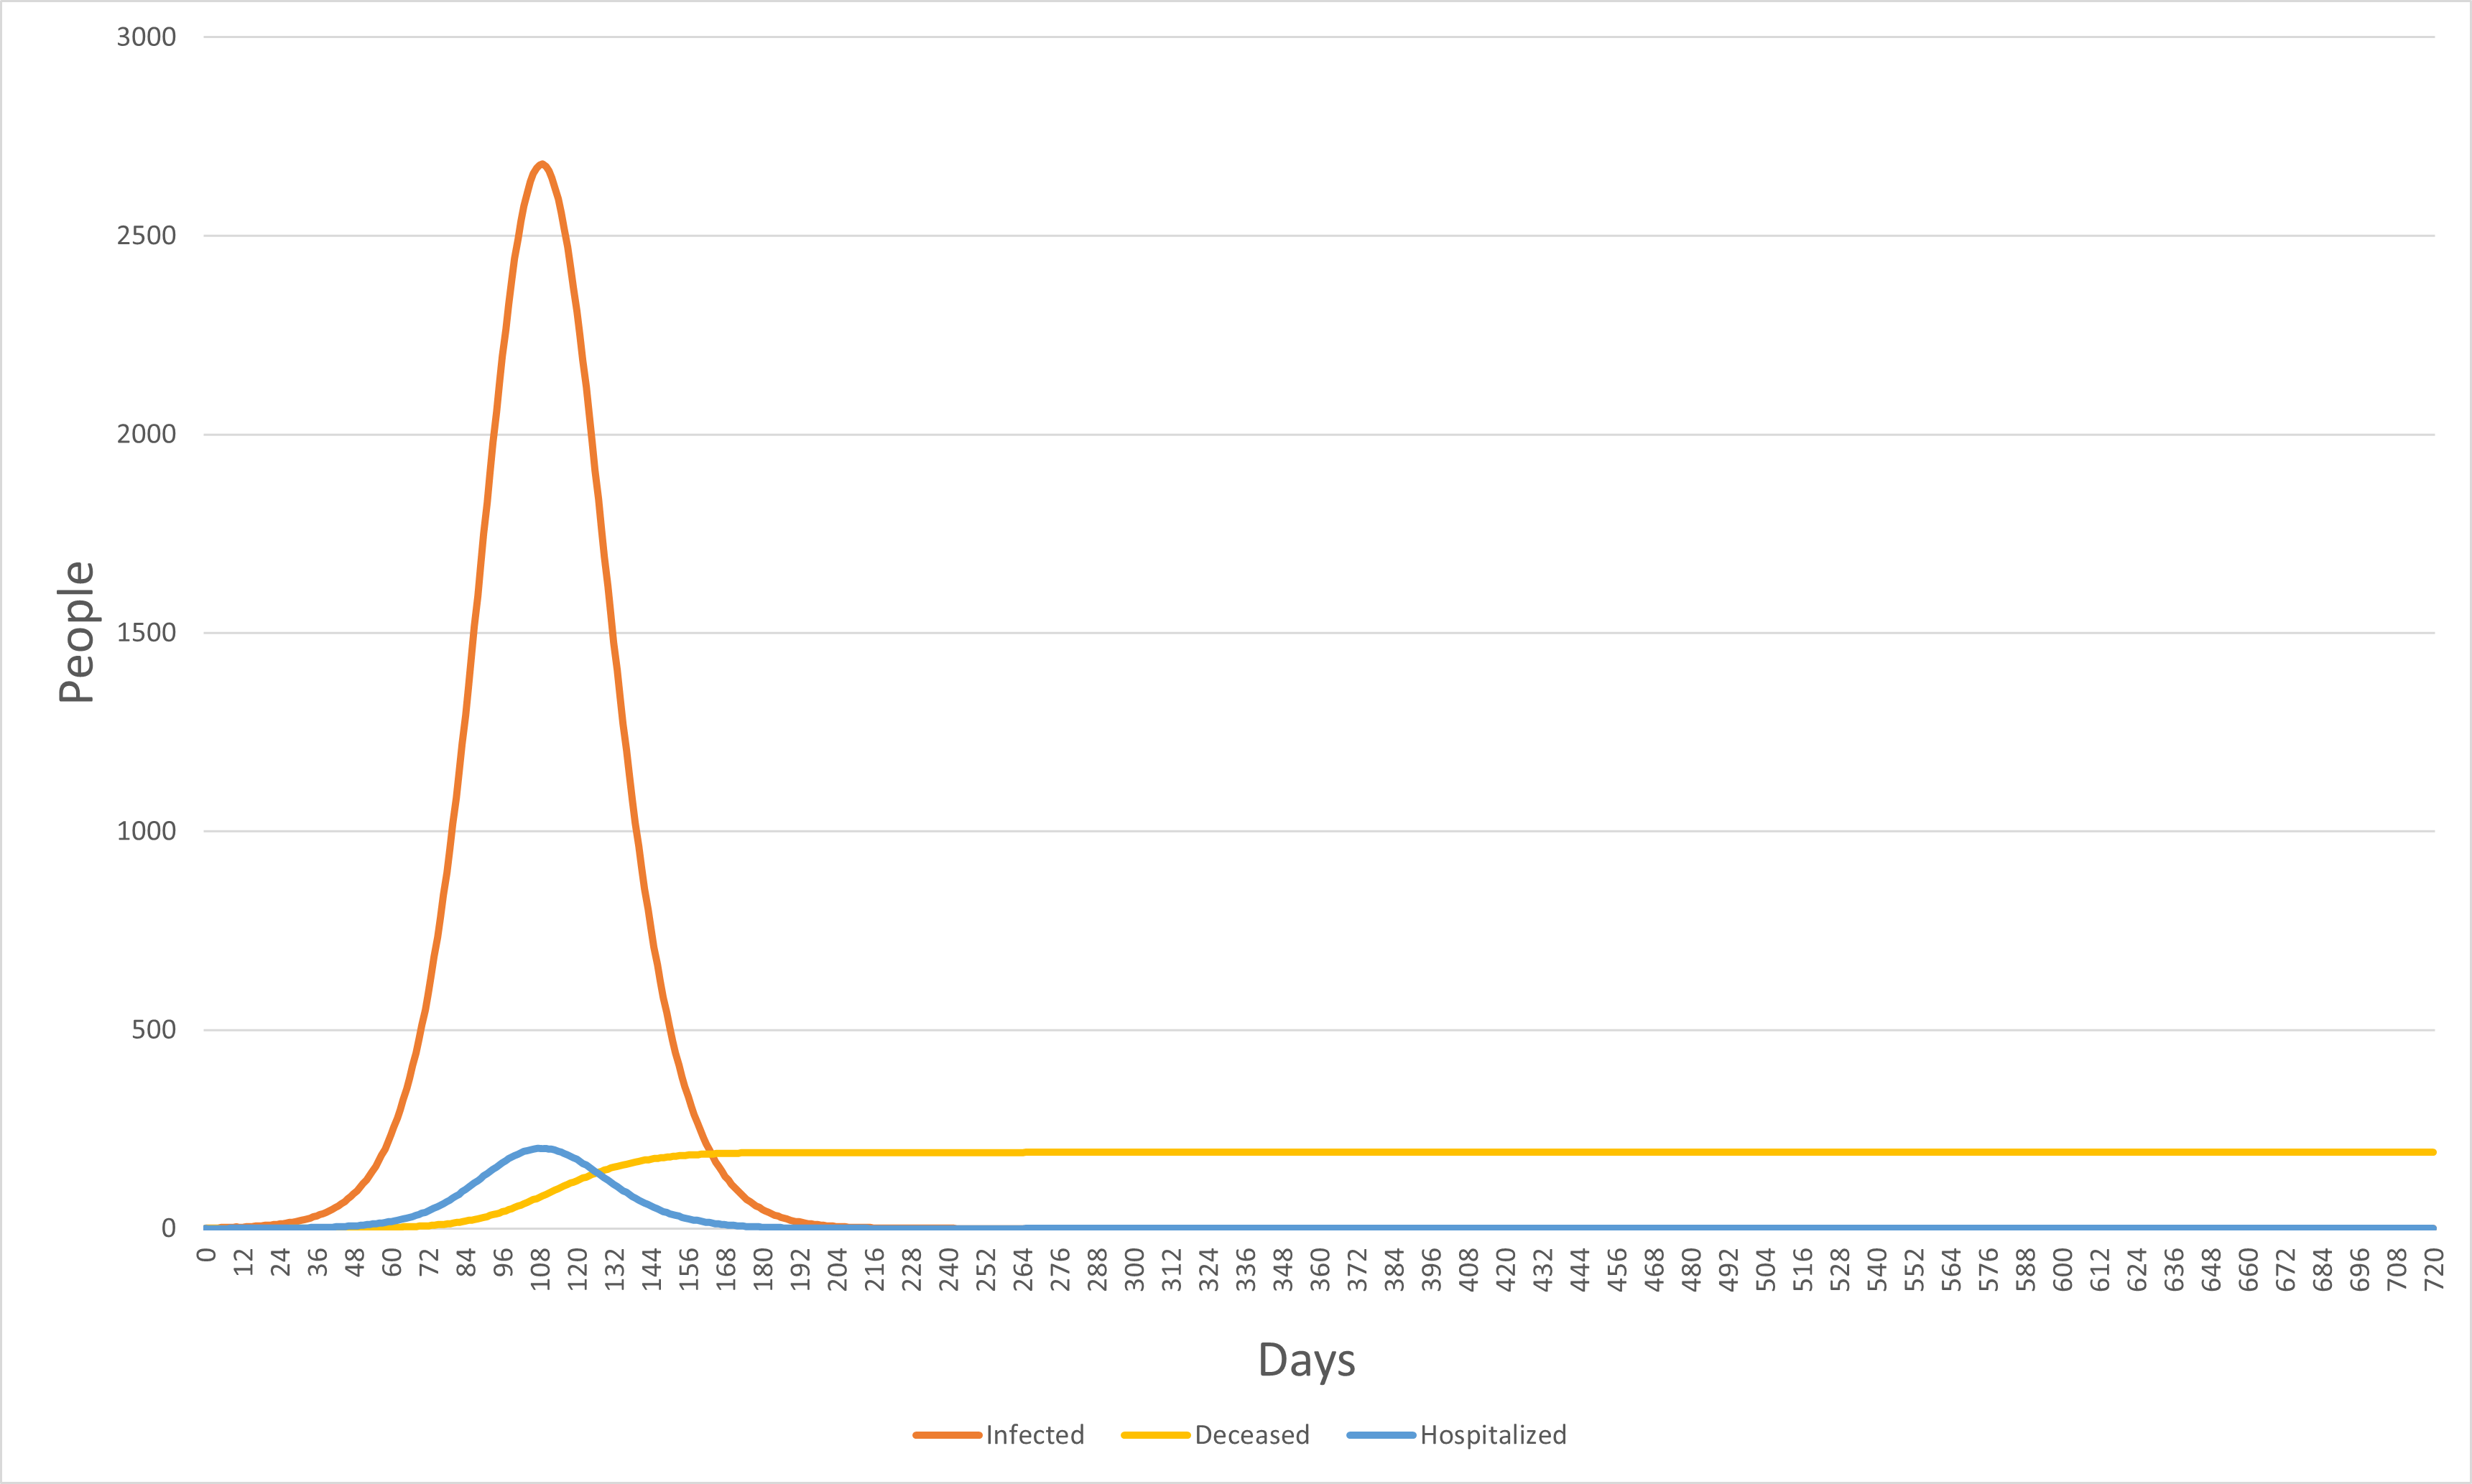
\includegraphics[width=.95\linewidth]{0_billeder/covidInfectionGraphA.png}
    \caption{With contact tracing}
    \label{Subfig:covidInfGraphA}
  \end{subfigure}
  \begin{subfigure}{.45\textwidth}
    \centering
    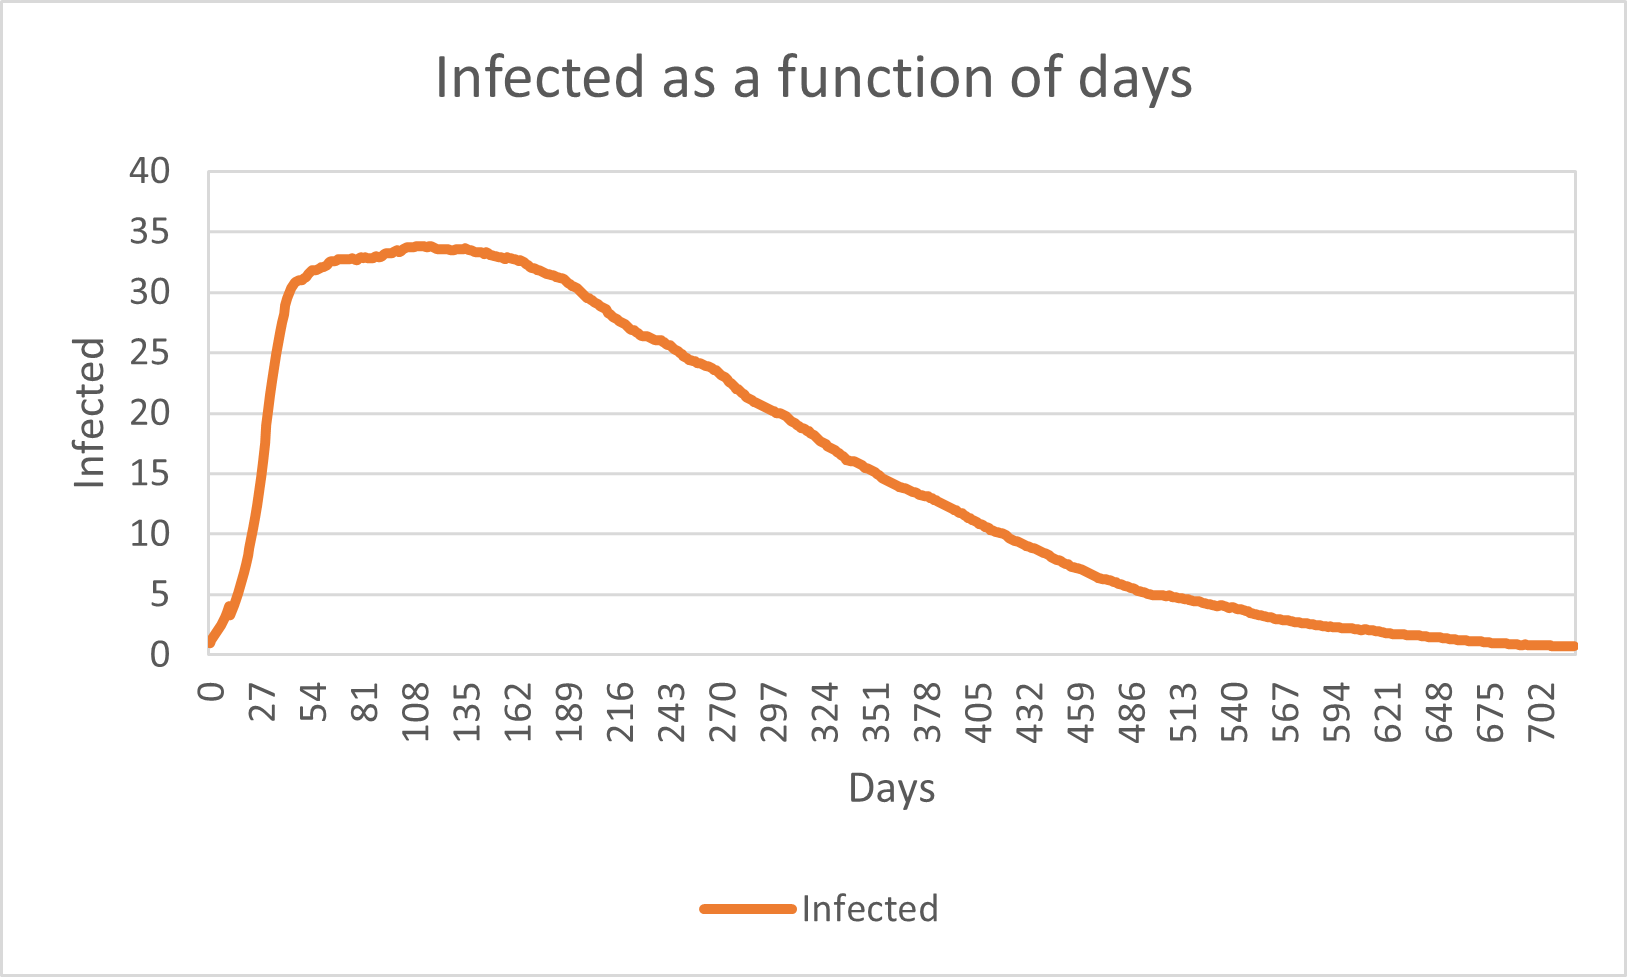
\includegraphics[width=.95\linewidth]{0_billeder/covidInfectionGraphB.png}
    \caption{Without contact tracing}
    \label{Subfig:covidInfGraphB}
  \end{subfigure}
 \caption{Infection graphs with and without contact tracing.}
 \label{Fig:covidInfGraphs}
\end{figure}
